\section{Digital Library}
Shady websites have long managed to monetize content downloads.
To provide free access to papers, we can follow their model by making the
following changes.

\subsection{Fake Download Buttons}

Fake download buttons are a staple of modern download websites. They really class up the web. Reifying, elegizing, and idealizing nature, these abstract forms with rococo garnishes direct the downloader's attention away from the url to the ad-serving service to which the button points. A deceptive d\'{e}tournement, the premonitory placement of these blissed-out buttons challenges browsers to consider whether they really want to download the paper -- they could, after all, not pursue their line of inquiry and instead watch it evolve vicariously -- which cuts down on the ACM's hosting costs.

By allowing advertisers to buy space on our digital library with which to
create ads that look like download buttons, advertisers can deceive users into
clicking an ad.
The advertiser and the ACM both profit off of these deceptive ads as the user
is redirected to see the advertiser's product while the ACM gets the revenue
for an impression. Some regulators have questioned this practice. But we believe it is a win-win-win for consumers \footnote{Gary Cohn, the director of the National Economic Council, stressed in an interview with *The Wall Street Journal* compared a website without fake-download buttons to the menu at P.J. Bland's: ``This is like putting only health food on the menu, because unhealthy food tastes good. But you still shouldn?t eat it because you might die younger." The menus of a free society, in his reckoning, should include both unhealthy and healthy items, and they should be labeled and priced identically. It should be impossible for consumers to access independent, third-party statistics about menu items. ``We believe our customers are informed and engaged, and we trust that they are smart enough to make the decisions that are right for them. We don't want the government treating them like dotards," the Gary Cohns said in unison.}.


Additionally, these download buttons could be functional in that they download
\textit{something}, but the ACM digital library will not impose any
restrictions on what may be downloaded from these fake buttons.
Therefore, advertisers are welcome to serve us infected PDFs or straight up
executables.
It is our position that users must be intelligent enough to hunt down the
proper download button, and that academics can learn valuable security
practices when they know that others could steal their research through
malicious downloads on the digital library.

To subvert ad blockers, the ad content will be natively hosted on the ACM
digital library as well.
Therefore, ad blockers will be unable to determine which requests are ad
related.

Lastly, we are revolutionizing the fake download practice by dynamically
randomizing the position of the actual download button.
Like serving ad content natively, this will make ad blockers functionally
useless as there will be no way to differentiate between ad content and ACM
content, providing users with instruction on the contingency of fate.
Moreover, this randomization makes it much harder for the user to learn the
positioning of the ads and therefore we hope to drive more clicks to our ad
partners and generate more revenue for the ACM.

\subsection{Rate Limited Free Downloads}
Free download sites figured out long ago that you can make people pay for an
otherwise free product by making the process of obtaining that free product
difficult.
Therefore, we will split our digital library downloads into two tiers, the free
tier and the \premium tier.

The free tier will only allow downloads at \todo{rate} and no more than one
paper download per day.
Additionally, the user will be required to watch an upgrade screen
\todo{explain this} count down for 10 minutes before the download button is
clickable.
If the website loses focus, the counter will be restarted.
The \premium tier will cost \todo{rate} but will allow unlimited downloads and
will not be rate limited.


\subsection{Outsourced Captias}
\todo{Force free-tier users to solve a captia, but the captia is actually from
  another site and we collect money from spammers to solve these captias ala
mechanical turk}

\subsection{ACM Digital Library Toolbar}
Like Java, every ACM paper will come as an executable.
Running this executable will ``install" the paper to the users desktop.
The only purpose of the install is to push the ACM Digital Library toolbar.
While the toolbar itself is optional, its installation is opt-out.
The ACM DL toolbar will be installed for all of the users web browsers where it
will follow them from site to site collecting information about their browsing
habits.
We will then sell this information to advertisers.

Additionally, the toolbar will constantly mine bitcoins on the user's machine
and send the mined coins to the ACM's wallet.
If the user has a GPU, the development drivers will be silently installed along
with the toolbar to enable GPU mining.
We hope that one day the ACM mining pool becomes so large that we become a
dominant player in the Bitcoin economy.
If we ever reach a simple majority of the mining power, we WILL mount a 51\%
attack to seize control of the network for our own financial gain.

\subsection{Impact Factor-ometer}

Researchers want their projects to have meaning and impact. Administrators like to market their department's product as meaningful and impactful. But how can researchers tell their work is saving the world?

Simple. Once a quarter, the Ricketts family convokes Gary Cohn, Dennis Rodman, Colonel Sanders, and the rest of the Economic Advisory Council at Chicago's historic Wrigley Field to make use of the stadium's native Noise-ometer. As Pat Hughes reads the papers over the PA in a Charlie Brotman accent, the council---taking especial care to note the presence of key phrases like ``cross-promotional deal mechanics revenue streams jargon synergy" and ``a strategic planning initiative\ldots with a focus on strategic dynamism"---emits cheers in proportion to its perception of the paper's impact, and these cheers are registered on the Noise-ometer, which assigns metrics of impact to each paper, as shown in Figure \todo{fig:noiseometer}

\begin{figure}
  \centering
  %https://archive.org/details/414803main_0203243
  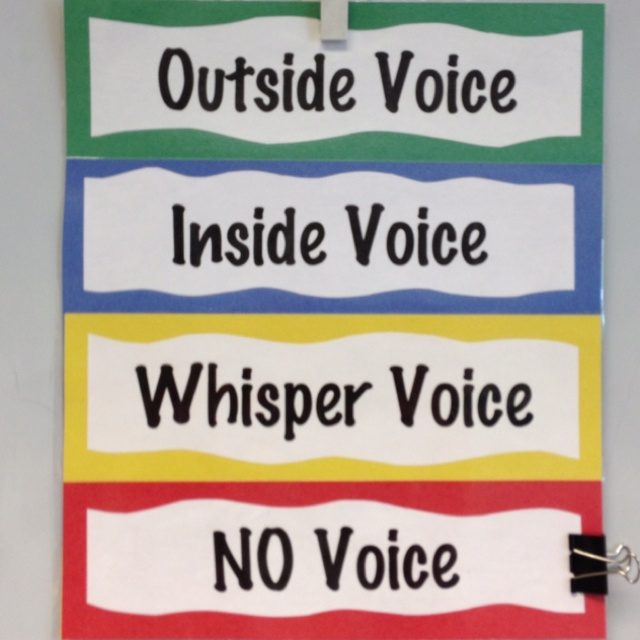
\includegraphics[width=0.45\textwidth]{figures/noiseometer.jpg}
  \caption{A model-year 1985 Noisome-ter, prized by collectors for its muted design that limns adumbrations of sound. The paper in which these meetings were proposed was met at the first such convening of the Council with a cheer so loud it registered a ``Fuck Yeah!" (not shown) on this scale.}
  \label{fig:noiseometer}
\end{figure}

These metrics empower our research partners to be certain their research is having a real-world impact.  It is important for researchers to know that they don't risk deactivation or exile if they remain on track.